\documentclass[10pt,letterpaper,fleqn]{article}

\usepackage[utf8]{inputenc}
\usepackage[spanish,es-nodecimaldot]{babel}
\usepackage{amsmath}
\usepackage{amssymb}
\usepackage{multicol}
\usepackage{graphicx}
\usepackage{mdwlist}

\usepackage[dvipsnames]{xcolor}
\usepackage[most]{tcolorbox}

\usepackage{tabu}

\usepackage{mathtools}

\usepackage[top=1in, bottom=1in, left=1in, right=1in]{geometry}


\begin{document}

\begin{titlepage}
    \centering

    {\scshape\LARGE Universidad Nacional Autónoma de México \par}

    \vspace{1cm}
    {\scshape\Large Facultad de Ciencias\par}
    \vspace{1.5cm}

    \begin{center}
        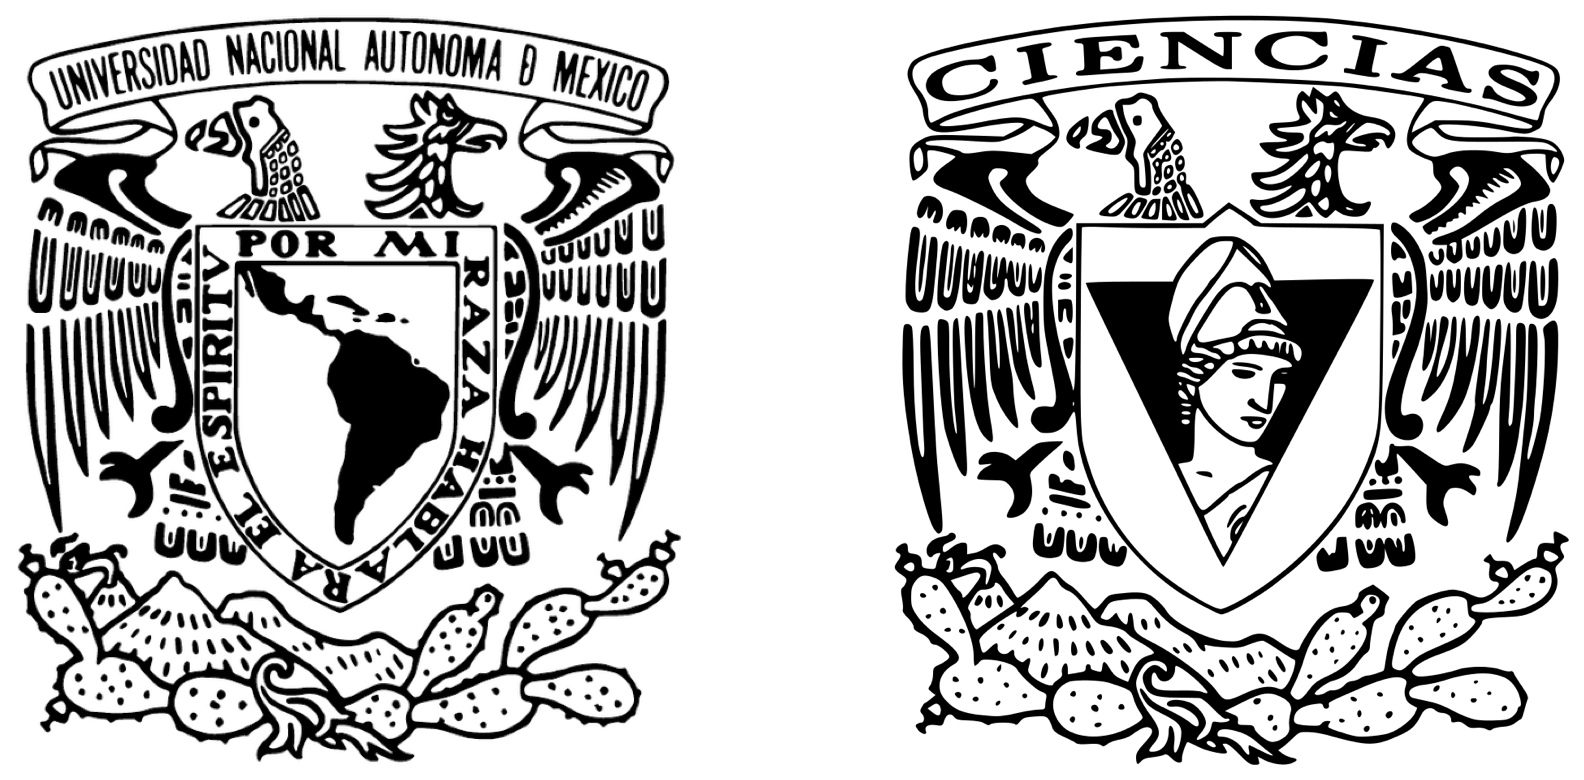
\includegraphics[scale=.1]{assets/img/logo.png}
    \end{center}

    \vspace{.8 cm}

    {\LARGE Tarea 2: \par}
    {\huge\bfseries Ejercicios \par}

    \vspace{0.5cm}
    \large{\itshape{Luis Erick Montes Garcia}} \small{ - 419004547}\\
    \large{\itshape{Hele Michelle Salazar Zaragoza}} \small{ - 316068895}


    \vfill

    Trabajo presentado como parte del curso de
    \textbf{Matematicas Aplicadas para las Ciencias II}
    impartido por el profesor \textbf{Juan Carlos Balleza}. \par
    \vspace{0.1cm}
    {\large Entrega 3 de Abril 2019 \par}
    \footnotesize{\textbf{Link al código fuente:} git@github.com:lemg98/Matematicas-Aplicadas-II.git}
\end{titlepage}

    \begin{enumerate}
        %Ejercicio 1.
        \item 

        %Ejercicio 2.
        \item Sea la función vectorial $r (\overrightarrow{t}) = (4cos({t \over 2}),4sin({t \over 2}))$, donde $t \in [0,2\pi]$. A continuación responda lo siguiente:
        %Incisos del ejercicio 2.
        \begin{enumerate}
            %Inciso a
            \item Calcule los vectores de velocidad y aceleración.
            \\ Obtenemos la derivada de la función  $r (\overrightarrow{t})$ para obtener la {\bf velocidad}: 
            \begin{center}
                $r'(\overrightarrow{t}) = (-2sin({t \over 2}),2cos({t \over 2}))$ 
            \end{center}

            Obtenemos la derivada de la función $r'(\overrightarrow{t})$ para obtener la {\bf aceleración}:
            \begin{center}
                $r''(\overrightarrow{t}) = (-cos({t \over 2}),-\sin({t \over 2}))$ \\
                \begin{tabular}{|c|c|c|} \hline 
                    t & velocidad & aceleración \\ \hline
                    $0$ & $(0,2) $ & $(-1,0)$  \\ \hline
                    $2\pi$ & $(-0.109,1.99)$ & $(-0.99,-0.054)$  \\ \hline
                \end{tabular}
            \end{center}

            %Inciso b
            \item Grafique la función vectorial, en el intervalo de $t$ indicado.
            \begin{center}
                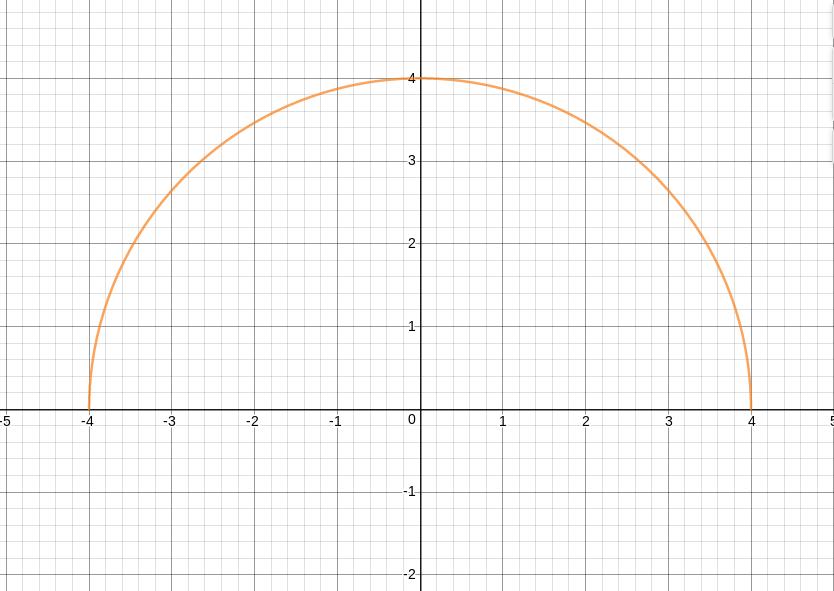
\includegraphics[scale=.3]{assets/img/ejercicio2(b).png}
            \end{center}
            %Inciso c
            \item En la gráfica de la función vectorial (inciso anterior), agregue los vectores de velocidad y aceleración en el instante $t = \pi$ 
            \begin{center}
                \begin{tabular}{|c|c|c|} \hline 
                    t & velocidad & aceleración \\ \hline
                    $\pi$ & $(-0.054,1.99) $ & $(-0.99,-0.02)$  \\ \hline
                \end{tabular}
                \\
                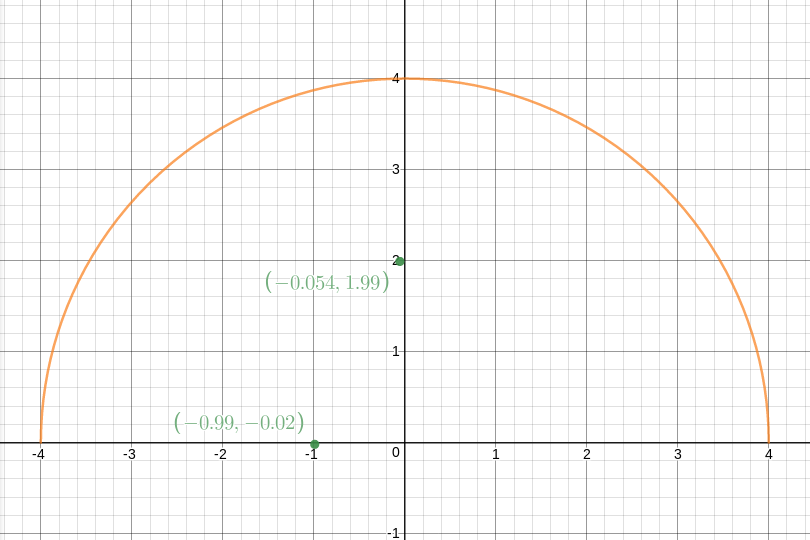
\includegraphics[scale=.3]{assets/img/ejercicio2(c).png}
            \end{center}

            %Inciso d
            \item Obtenga el ángulo entre los vectores velocidad y aceleración.
            \\ Decimos que el vector de velocidad es el vector $\overrightarrow{a}$ y que el vector de aceleración es $\overrightarrow{b}$. Para obtener el ángulo $\theta$ formamos un triángulo, siendo $\overrightarrow{a}-\overrightarrow{b}$ el lado opuesto al ángulo.
            \\ Aplicando ley de cosenos, tenemos que: \\
            $$(\overrightarrow{a} \cdot \overrightarrow{b})=||\overrightarrow{a}|| ||\overrightarrow{b}|| \cos \theta $$ \\
            Despejamos $\Cos \theta$: \\
            $$\cos \theta = {(\overrightarrow{a} \cdot \overrightarrow{b}) \over ||\overrightarrow{a}|| ||\overrightarrow{b}||}$$ \\ 
            Sustituímos: \\
            $$\cos \theta = {((-0.054,1.99) \cdot (-0.99,-0.02)) \over ||(-0.054,1.99)|| ||(-0.99,-0.02)||}$$ \\
            $$\cos \theta = {((-0.054 \cdot-0.99) + (1.99 \cdot -0.02)) \over \sqrt{(-0.054)^2 + (1.99)^2} \cdot \sqrt{(-0.99)^2 + (-0.02)^2}}$$ \\
            $$\cos \theta = {0.09326 \over (1.99)(0.99)}$$ \\
            $$\cos \theta = {0.09326 \over 1.9701}$$ \\
            $$\cos \theta = {0.04733}$$ \\
            Sacamos coseno inverso: \\
            $$\theta = \cos^-1 (0.04733) = 87.29 \delta$$

        \end{enumerate}


        %Ejercicio 3.
        \item

        %Ejercicio 4.
        \item Proporcione la función vectorial $r(\overrightarrow{t})$, tal que cumpla las siguientes condiciones:
        %Incisos del Ejercicio 4.
        \begin{enumerate}
            %Inciso a
            \item $a(t)=(-1,-1,-1)$ \\
            $x = 0-t$ ; $y = 0-t$ ; $ z = 0-t$ y $0 \leqslant t \leqslant 1$\\
            $(x,y,z)=(0-t,0-t,0-t)$ \\
            $(x,y,z)=(0,0,0)+(-t,-t,-t)$ \\
            $(x,y,z)=(0,0,0)+t(-1,-1,-1)$ \\
            $a=(0,0,0)+t(-1,-1,-1)$ 
            %Inciso b
            \item $v(0)=(0,0,0)$

            %Inciso c
            \item $r(0)=(10,10,10)$ \\
            $x=10$ ; $y=10$ ; $z=10$ \\
            $(x,y,z) = (10+0t,10+0t,10+0t)$ \\
            $(x,y,z) = (10,10,10)+(0t,0t,0t)$ \\
            $(x,y,z) = (10,10,10)+t(0,0,0)$ \\ 
            $v = (10,10,10)+t(0,0,0)$

        \end{enumerate}

        %Ejercicio 5.
        \item

        %Ejercicio 6.
        \item Considere la función vectorial $r(\overrightarrow{t})= ([\cos t]^3,[\sin t]^3)$. Responda lo siguiente:
        %Incisos del Ejercicio 6.
        \begin{enumerate}
            %Inciso a
            \item Obtenga el vector tangente unitario a la curva. \\
            Parametrizamos la función:
            $r(\overrightarrow{t})= ([\cos t]^3,[\sin t]^3)$ \\
            $\begin{bmatrix}
            {d \over dt} \cos^3 t \\
            {d \over dt} \sin^3 t \\
            \end{bmatrix}$ \\
            Encontramos un vector tangente: \\
            $\begin{bmatrix}
            -3sin(t)\cos^2(t) \\
            3sin^2(t)\cos(t) \\
            \end{bmatrix}$ \\
            Hacemos negativa la segunda componente para girar 90 grados en sentido de las manecillas del reloj. \\
            $\begin{bmatrix}
            3sin^2(t)\cos(t) \\
            -(-3sin(t)\cos^2(t))\\
            \end{bmatrix}$ \\
            Tenemos un vector normal, para hacerlo unitario, debemos dividir entre su magnitud, es decir, \\
            $$\sqrt{9sin^2(t)\cos^4(t)+9sin^4(t)\cos^2(t)}$$ \\
            Por lo tanto, la función para el vector unitario es el siguiente: \\
            $\begin{bmatrix}
            3sin^2(t)\cos(t) / \sqrt{9sin^2(t)\cos^4(t)+9sin^4(t)\cos^2(t)} \\
            3sin(t)\cos^2(t) / \sqrt{9sin^2(t)\cos^4(t)+9sin^4(t)\cos^2(t)}\\
            \end{bmatrix}$ \\
            %Inciso b
            \item Calcule la longitud de la curva para $t \in [0,{\pi \over 2}]$ \\
            $$\sqrt{9sin^2(t)\cos^4(t)+9sin^4(t)\cos^2(t)}$$ \\
            Sustituímos: \\
            $$\sqrt{9sin^2(0)\cos^4(0)+9sin^4(0)\cos^2(0)} = 0$$ \\
            $$\sqrt{9sin^2({\pi \over 2})\cos^4({\pi \over 2})+9sin^4({\pi \over 2})\cos^2({\pi \over 2})} = 0$$
        \end{enumerate}

        %Ejercicio 7.
        \item

        %Ejercicio 8.
        \item Obtenga la ecuación del círculo osculador para la función $y=\sin x$ en el punto de coordenadas $({\pi \over 2},1)$. Proponga $r(\overrightarrow{t})$ a partir de la "parametrización trivial" de la función. Calcule lo siguiente: 
        %Incisos del Ejercicio 8.
        \begin{enumerate}
            \item $(\overrightarrow{T})$, $(\overrightarrow{N})$ y $k$.\\
            Parametrización de la función: \\
            $x(t) = t \\
             y(t) = \sin t$
        \end{enumerate}
        Haga una gráfica con la siguiente información:
        \begin{enumerate}
            \item La función $y=\sin x$ \\
            \begin{center}
                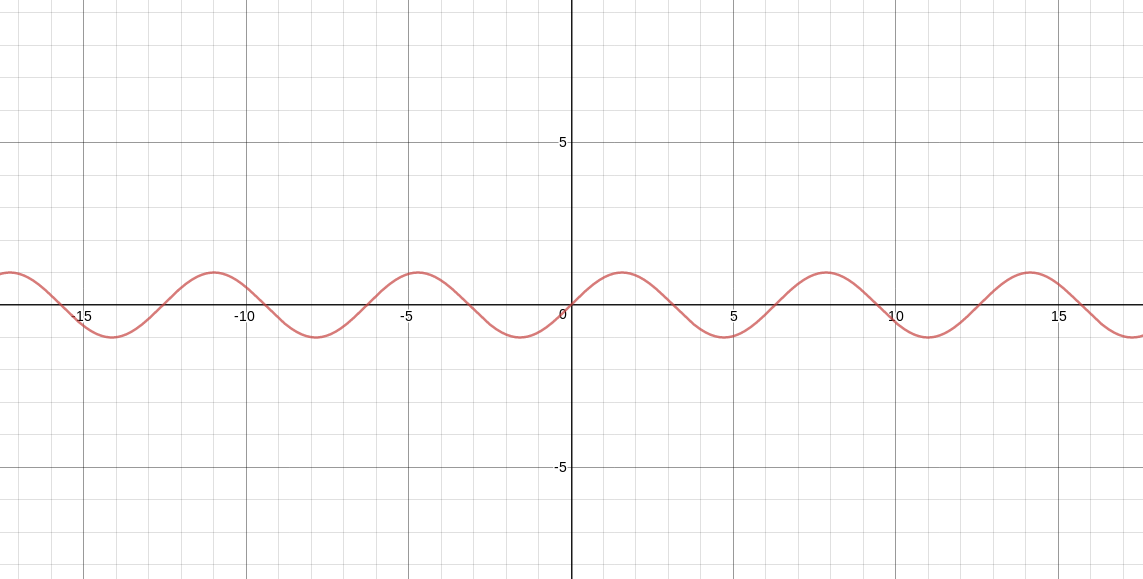
\includegraphics[scale=.3]{assets/img/ejercicio8(b).png}
            \end{center}
            \item El círculo osculador y además localizar el punto de coordenadas $({\pi \over 2},1)$
            \item Los vectores $(\overrightarrow{T})$, $(\overrightarrow{N})$.
        \end{enumerate}

        %Ejercicio 9
        \item 


    \end{enumerate}





\end{document}